\begin{center}
    {\Large\bfseries Решения задач}
\end{center}

% Источник задачи: Турнир городов, международный (архив Торонто), весна 2012, старшая группа, сложный вариант (A-level), задача № 1; https://www.math.toronto.edu/oz/turgor/archives/TT2012S_SAsolutions.pdf
% Источник решения: официальное решение Турнира городов; https://www.math.toronto.edu/oz/turgor/archives/TT2012S_SAsolutions.pdf

\problem{1}
\textit{В отряде охранников каждому назначено своё натуральное число. Для любых двух охранников отношение большего из назначенных им чисел к меньшему не меньше $3$. Охранник, которому назначено число $n$, дежурит $n$ дней подряд, затем $n$ дней подряд отдыхает, затем снова дежурит $n$ дней подряд и так далее. Начинать дежурства охранники могут в разные дни. Возможно ли устроить графики так, чтобы каждый день дежурил хотя бы один охранник?}

\textbf{Ответ:} нет.

\textbf{Решение.}
Пусть назначенные числа, выписанные в порядке убывания, равны
\[
 n_1>n_2>\dots>n_s\geq1.
\]
Из условия следует $n_i\geq3n_{i+1}$ для каждого $i<s$.

У первого охранника имеются промежутки отдыха длины $n_1$, поэтому внутри одного из них можно выбрать $3n_2$ последовательных дней. Рассмотрим любой промежуток из $3n_2$ последовательных дней. У второго охранника периоды дежурства и отдыха имеют длину $n_2$. Такой промежуток обязательно содержит целый период его отдыха длины $n_2$: действительно, от начала промежутка до ближайшего начала периода отдыха проходит меньше $2n_2$ дней, после чего остаётся не менее $n_2$ дней.

Итак, внутри выбранного промежутка найдётся промежуток длины $n_2$, когда не дежурят уже первые два охранника. Так как $n_2\geq3n_3$, внутри него тем же рассуждением найдётся промежуток длины $n_3$, когда не дежурят первые три. Продолжая, получим $n_s$ последовательных дней, когда не дежурит никто. Следовательно, покрыть дежурствами все дни невозможно.

% Источник задачи: Турнир городов, международный (архив Торонто), весна 2012, старшая группа, сложный вариант (A-level), задача № 2; https://www.math.toronto.edu/oz/turgor/archives/TT2012S_SAsolutions.pdf
% Источник решения: официальное решение Турнира городов; https://www.math.toronto.edu/oz/turgor/archives/TT2012S_SAsolutions.pdf

\problem{2}
\textit{Внутри круга отмечены $100$ точек, никакие три из которых не лежат на одной прямой. Докажите, что точки можно разбить на $50$ пар так, чтобы $50$ прямых, проходящих через точки каждой пары, попарно пересекались внутри круга.}

\textbf{Решение:}
Рассмотрим все разбиения данных точек на пары. Их конечное число, поэтому существует разбиение, для которого сумма длин $50$ соединяющих отрезков максимальна. Докажем, что оно подходит.  Предположим противное: две прямые, заданные парами $\{A,B\}$ и $\{C,D\}$, пересекаются вне круга (случай параллельных прямых рассматривается так же). Тогда четыре точки являются вершинами выпуклого четырёхугольника, а $AB$ и $CD$ --- его противоположными сторонами. Действительно, если одна точка лежала бы внутри треугольника трёх остальных, то прямая через неё и одну вершину пересекла бы противоположную сторону внутри этого треугольника, а значит, внутри круга.

Перенумеруем вершины в циклическом порядке как $A,B,C,D$ и обозначим через $E$ точку пересечения диагоналей $AC$ и $BD$. Она лежит внутри четырёхугольника, а значит, внутри круга.

По строгому неравенству треугольника
\[
 AB<AE+EB,\qquad CD<CE+ED.
\]
Следовательно,
\[
 AB+CD<AC+BD.
\]
Если заменить пары $\{A,B\}$ и $\{C,D\}$ парами $\{A,C\}$ и $\{B,D\}$, получится новое разбиение на пары с большей суммой длин. Это противоречит выбору исходного разбиения. Значит, любые две из выбранных прямых пересекаются внутри круга.

% Источник задачи: 62-я Международная математическая олимпиада, международная (Санкт-Петербург, Россия), 2021, шорт-лист, задача A3; https://www.imo-official.org/problems/IMO2021SL.pdf
% Источник решения: официальное решение шорт-листа IMO 2021, Solution 2 (идея покрытия степеней двойки); https://www.imo-official.org/problems/IMO2021SL.pdf

\problem{3}
\textit{Пусть $n$ --- натуральное число. Найдите наименьшее возможное значение суммы
\[
  \left\lfloor\frac{a_1}{1}\right\rfloor+
  \left\lfloor\frac{a_2}{2}\right\rfloor+\dots+
  \left\lfloor\frac{a_n}{n}\right\rfloor,
\]
где $(a_1,a_2,\dots,a_n)$ пробегает все перестановки чисел $1,2,\dots,n$.}

\textbf{Ответ:} $\lfloor\log_2 n\rfloor+1$

\textbf{Решение.} Положим $k=\lfloor\log_2 n\rfloor$, то есть $2^k\leq n<2^{k+1}$. Ответ равен
\[
  \boxed{k+1=\lfloor\log_2 n\rfloor+1}.
\]

Сначала построим перестановку, дающую это значение. Разобьём множество индексов на блоки
\[
 [1,1],\ [2,3],\ [4,7],\dots,\ [2^{k-1},2^k-1],\ [2^k,n].
\]
В каждом блоке $[p,q]$ положим
\[
 (a_p,a_{p+1},\dots,a_q)=(q,p,p+1,\dots,q-1).
\]
Так как $q<2p$, первый член блока даёт $\lfloor q/p\rfloor=1$, а каждый следующий член даёт $\lfloor(i-1)/i\rfloor=0$. Поэтому вклад каждого из $k+1$ блоков равен $1$.

Докажем нижнюю оценку. Назовём индекс $i$ хорошим, если $a_i\geq i$, и сопоставим ему целочисленный отрезок $[i,a_i]$.  Докажем, что хорошие отрезки покрывают все числа $1,\dots,n$. Зафиксируем $x\in\{1,\dots,n\}$ и предположим, что $x$ не принадлежит
ни одному из этих отрезков. Тогда для каждого $i\leq x$ должно
выполняться $a_i<x$: действительно, если бы $a_i\geq x$, то $i\leq x\leq a_i,$ откуда $x\in[i,a_i]$.

Таким образом, $x$ различных чисел $a_1,a_2,\dots,a_x$ принадлежат множеству $\{1,2,\dots,x-1\}$, содержащему всего $x-1$ элементов. Противоречие.

Следовательно, для каждого $x$ существует индекс $i$ такой, что $i\leq x\leq a_i.$ Значит, рассматриваемые отрезки покрывают все числа $1,\dots,n$.

В частности, хорошие отрезки покрывают $k+1$ чисел
\[
 1,2,4,\dots,2^k.
\]
Если отрезок $[i,a_i]$ содержит $r$ степеней двойки, то при $r\geq1$
\[
 \frac{a_i}{i}\geq 2^{r-1}\geq r,
\]
а потому $\lfloor a_i/i\rfloor\geq r$. Сумма величин $\lfloor a_i/i\rfloor$ по всем индексам не меньше общего числа покрытых степеней двойки, то есть не меньше $k+1$. Нижняя оценка совпала с построением.

% Источник задачи: 62-я Международная математическая олимпиада, международная (Санкт-Петербург, Россия), 2021, шорт-лист, задача G1; https://www.imo-official.org/problems/IMO2021SL.pdf
% Источник решения: официальное решение шорт-листа IMO 2021, Solution 1; https://www.imo-official.org/problems/IMO2021SL.pdf

\problem{4}
\textit{Дан параллелограмм $ABCD$, причём $AC=BC$. Точка $P$ лежит на продолжении отрезка $AB$ за точку $B$. Описанная окружность треугольника $ACD$ вторично пересекает отрезок $PD$ в точке $Q$, а описанная окружность треугольника $APQ$ вторично пересекает отрезок $PC$ в точке $R$. Докажите, что прямые $CD$, $AQ$ и $BR$ проходят через одну точку.}

\textbf{Решение.}
\noindent\textbf{Общие замечания.}
Приведённые ниже предварительные рассуждения используются во всех решениях.

Поскольку
\[
AC=BC=AD,
\]
имеем
\[
\angle ABC=\angle BAC=\angle ACD=\angle ADC.
\]
Так как четырёхугольники $APRQ$ и $AQCD$ вписанные, получаем
\[
\angle CRA
 =180^\circ-\angle ARP
 =180^\circ-\angle AQP
 =\angle DQA
 =\angle DCA
 =\angle CBA.
\]
Следовательно, точки $A$, $B$, $C$ и $R$ лежат на некоторой окружности~$\gamma$.

\medskip

\noindent\textbf{Решение 1.}
Введём точку
\[
X=AQ\cap CD.
\]
Нам требуется доказать, что точки $B$, $R$ и $X$ коллинеарны.

Из вписанности четырёхугольника $APRQ$ следует
\[
\angle RQX
 =180^\circ-\angle AQR
 =\angle RPA
 =\angle RCX,
\]
где последнее равенство следует из параллельности $AB\parallel CD$.
Значит, точки $C$, $Q$, $R$ и $X$ также лежат на некоторой
окружности~$\delta$.

Используя окружности $\delta$ и $\gamma$, окончательно получаем
\[
\angle XRC
 =\angle XQC
 =180^\circ-\angle CQA
 =\angle ADC
 =\angle BAC
 =180^\circ-\angle CRB.
\]

\begin{figure}[h]
    \centering
    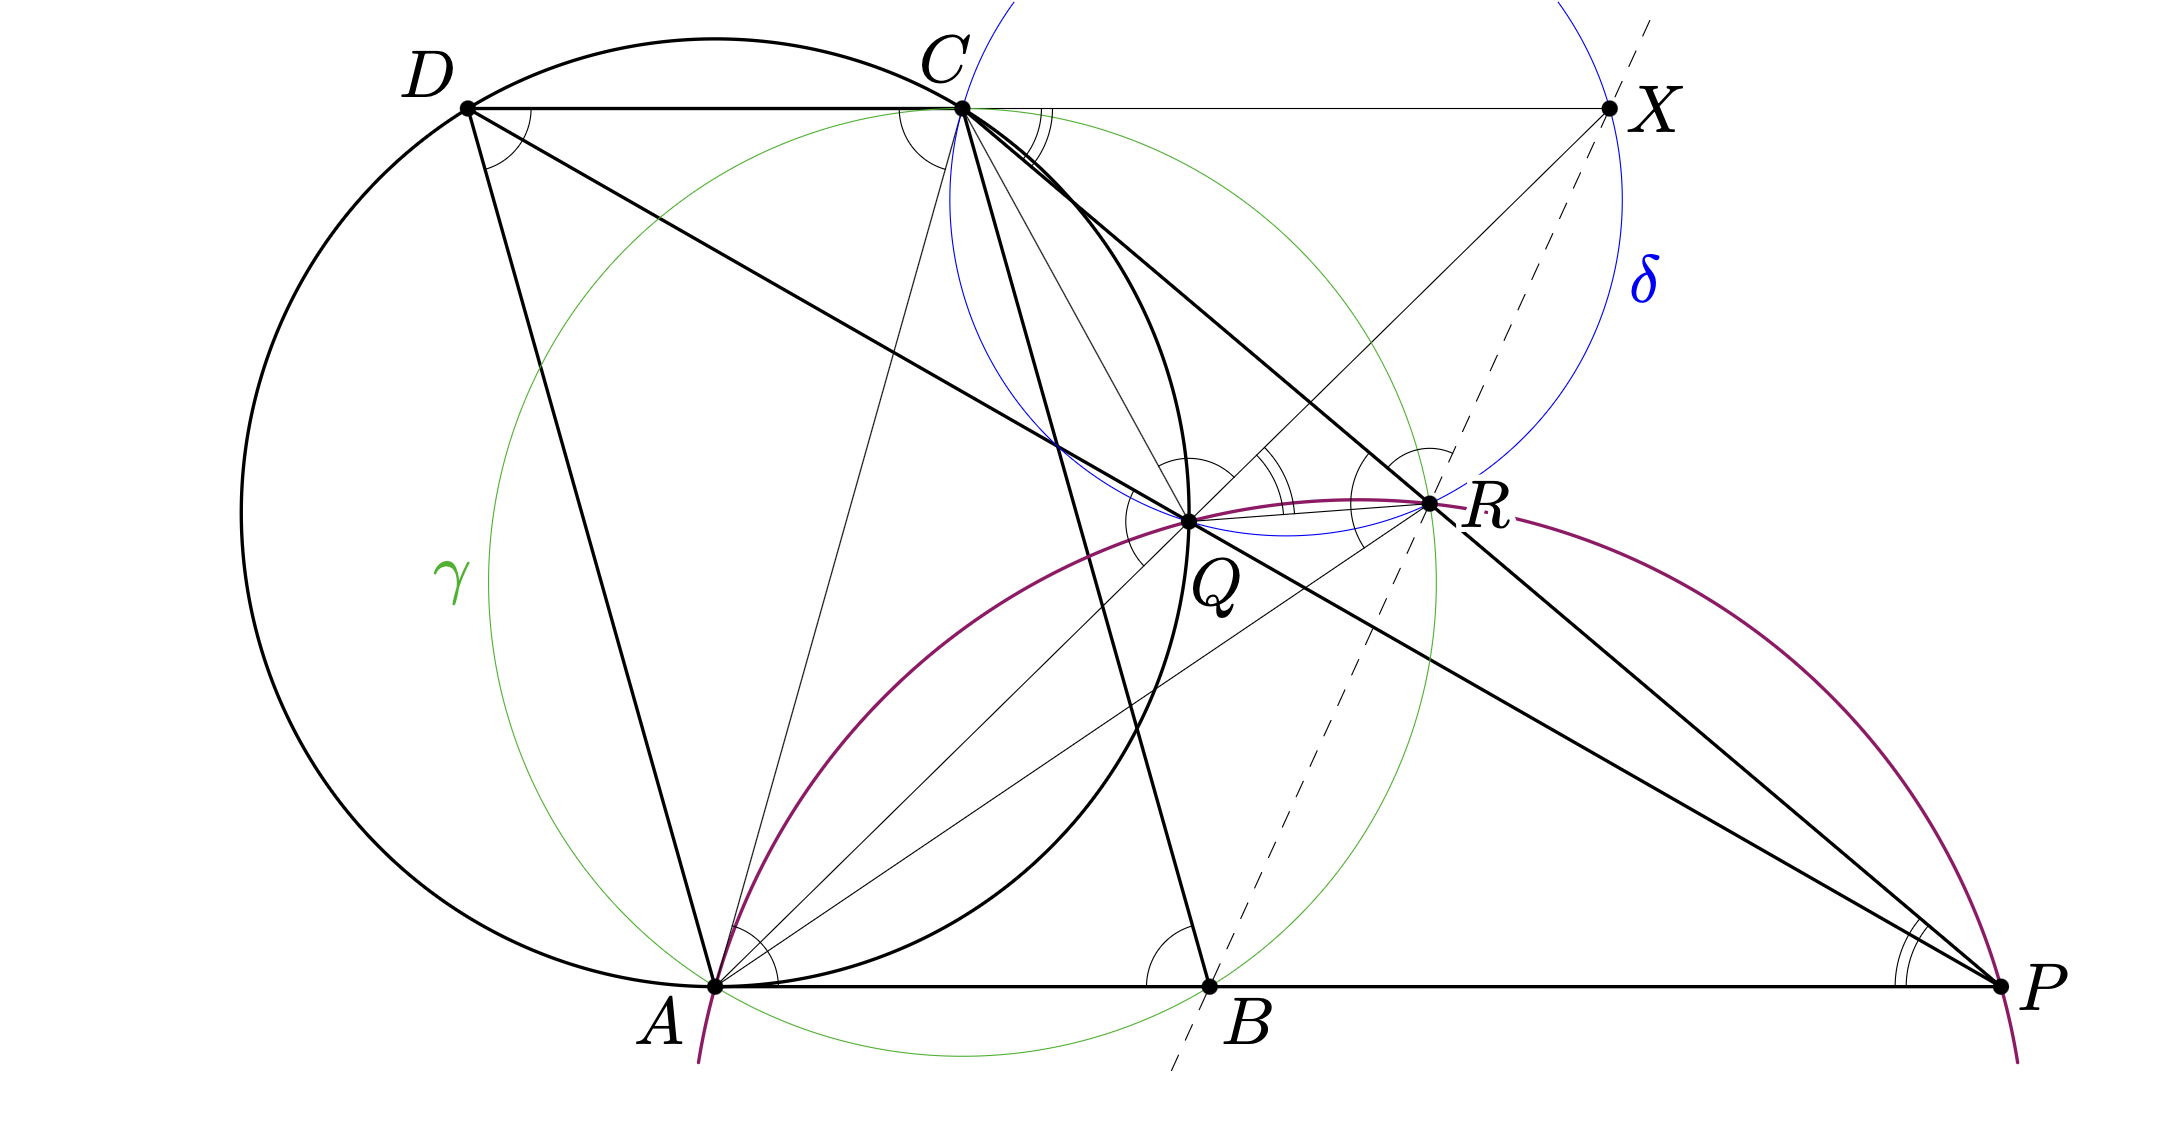
\includegraphics[width=1\linewidth]{Сборы//Сборы Элиста 2026//Алина Эльзята и Герман/turgor_4.1.png}
\end{figure}

Следовательно, точки $X$, $R$ и $B$ коллинеарны, что и требовалось
доказать.



\medskip

\noindent\textbf{Решение 2.}
Обозначим через $\alpha$ окружность $(APRQ)$. Поскольку
\[
\angle CAP
 =\angle ACD
 =\angle AQD
 =180^\circ-\angle AQP,
\]
прямая $AC$ касается окружности $\alpha$.

Пусть теперь прямая $AD$ вторично пересекает $\alpha$ в точке $Y$.
Эта точка обязательно лежит на продолжении луча $DA$ за точку $A$.
Используя окружность $\gamma$ и касание прямой $AC$ к окружности
$\alpha$, получаем
\[
\angle ARY
 =\angle CAD
 =\angle ACB
 =\angle ARB.
\]
Следовательно, точки $Y$, $B$ и $R$ коллинеарны.

Применим теорему Паскаля к вырожденному шестиугольнику $AAYRPQ$,
где прямая $AA$ понимается как касательная к окружности $\alpha$
в точке $A$. Тогда точки
\[
AA\cap RP=C,\qquad
AY\cap PQ=D,\qquad
YR\cap QA
\]
лежат на одной прямой. Следовательно, прямые $CD$, $AQ$ и $BR$
проходят через одну точку.

\medskip

\noindent\textbf{Замечание 1.}
Решение 2 состоит из двух частей:
\begin{enumerate}
    \item доказательства того, что прямые $BR$ и $DA$ пересекаются
    в точке окружности $\alpha$;
    \item доказательства того, что из этого следует требуемая
    конкурентность прямых.
\end{enumerate}
Решение 3 также разбивается на эти две части, однако доказательства
в них отличаются.

\begin{figure}[h]
    \centering
    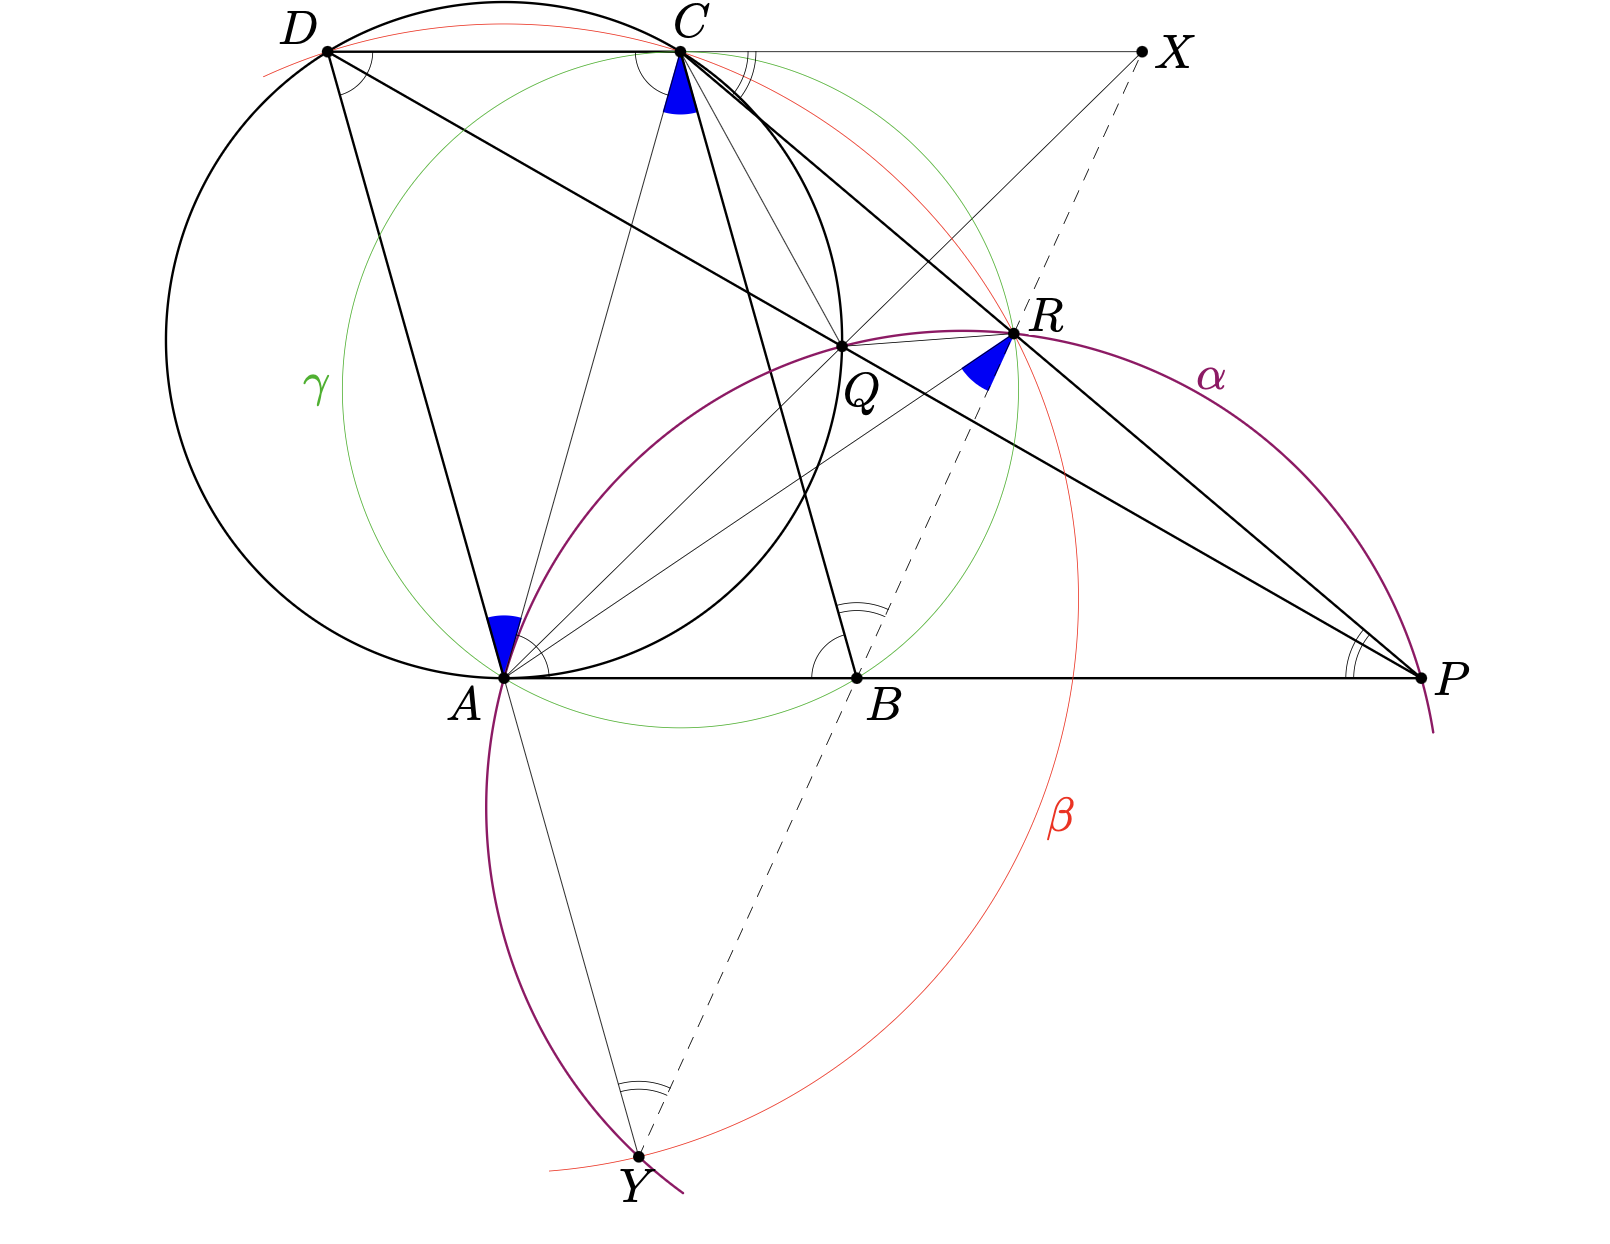
\includegraphics[width=1\linewidth]{Сборы//Сборы Элиста 2026//Алина Эльзята и Герман/turgor_4.2.png}
\end{figure}

\medskip

\noindent\textbf{Решение 3.}
Как и в решении 1, введём точку
\[
X=AQ\cap CD
\]
и докажем, что точки $B$, $R$ и $X$ коллинеарны. Как и в решении 2,
обозначим
\[
\alpha=(APQR),
\]
но теперь определим $Y$ как вторую точку пересечения прямой $RB$
с окружностью $\alpha$.

Используя окружность $\alpha$ и замечая, что прямая $CD$ касается
окружности $\gamma$, получаем
\begin{equation}
\angle RYA
 =\angle RPA
 =\angle RCX
 =\angle RBC.
\tag{1}
\end{equation}
Следовательно,
\[
AY\parallel BC,
\]
а потому точка $Y$ лежит на прямой $DA$.

Кроме того, цепочка равенств \textup{(1)} показывает, что
\[
\angle RYD=\angle RCX.
\]
Отсюда следует, что точки $C$, $D$, $Y$ и $R$ лежат на некоторой
окружности~$\beta$.

Таким образом, прямые $CD$, $AQ$ и $YBR$ являются попарными
радикальными осями окружностей $(AQCD)$, $\alpha$ и $\beta$.
Следовательно, эти три прямые проходят через одну точку.

% Источник задачи: 62-я Международная математическая олимпиада, международная (Санкт-Петербург, Россия), 2021, шорт-лист, задача N3; https://www.imo-official.org/problems/IMO2021SL.pdf
% Источник решения: официальное решение шорт-листа IMO 2021; https://www.imo-official.org/problems/IMO2021SL.pdf

\problem{5}
\textit{Найдите все натуральные числа $n$, обладающие следующим свойством: все $k$ натуральных делителей числа $n$ можно расположить в некотором порядке $d_1,d_2,\dots,d_k$ так, что при каждом $i=1,2,\dots,k$ сумма $d_1+d_2+\dots+d_i$ является точным квадратом.}

\textbf{Ответ:} $n=1$ или $n=3$.

\textbf{Решение.}
Пусть для некоторого подходящего порядка делителей
\[
 d_1+\dots+d_i=s_i^2\qquad (i=1,\dots,k),
\]
где также положим $s_0=0$. Частичные суммы строго возрастают, поэтому
\[
 0=s_0<s_1<\dots<s_k,\qquad s_i\geq i.
\]
Отсюда
\[
 d_i=s_i^2-s_{i-1}^2=(s_i-s_{i-1})(s_i+s_{i-1})
 \geq s_i+s_{i-1}\geq2i-1. \tag{1}
\]
Так как среди делителей есть $1$, из (1) следует $d_1=1$, а значит $s_1=1$.

Докажем по индукции, что
\[
 s_i=i,\qquad d_i=2i-1 \quad (i=1,\dots,k). \tag{2}
\]
База $i=1$ уже установлена. Предположим (2) для индексов до $i$ и рассмотрим $d_{i+1}$. Имеем
\[
 d_{i+1}=s_{i+1}^2-i^2=(s_{i+1}-i)(s_{i+1}+i).
\]
Число $d_{i+1}$ делит $n$, поэтому каждый из двух положительных целых множителей, в частности $s_{i+1}+i$, тоже делит $n$. Значит, $s_{i+1}+i=d_j$ для некоторого $j$.

Из (1) получаем $d_j\geq s_j+s_{j-1}$. Если бы $j>i+1$, то строгая монотонность последовательности $s_t$ дала бы
\[
 d_j\geq s_j+s_{j-1}>s_{i+1}+s_i=s_{i+1}+i,
\]
противоречие. Поэтому $j\leq i+1$. С другой стороны,
\[
 d_j=s_{i+1}+i>2i>d_i>d_{i-1}>\dots>d_1,
\]
так что $j$ не может быть не больше $i$. Следовательно, $j=i+1$ и
\[
 s_{i+1}+i=d_{i+1}=(s_{i+1}-i)(s_{i+1}+i).
\]
Сокращая на положительное число $s_{i+1}+i$, получаем $s_{i+1}-i=1$. Значит, $s_{i+1}=i+1$ и $d_{i+1}=2i+1$. Индукция завершена.

Таким образом, все делители $n$ в некотором порядке равны
\[
 1,3,5,\dots,2k-1.
\]
Если $k=1$, то $n=1$. Если $k\geq2$, то $n=2k-1$, а второй по величине делитель равен $n-2$; следовательно, $n-2\mid n$, откуда $n-2\mid2$. Число $n-2$ положительно и нечётно, поэтому $n-2=1$ и $n=3$.

Проверка: для $n=1$ порядок $(1)$ даёт сумму $1$; для $n=3$ порядок $(1,3)$ даёт частичные суммы $1$ и $4$.

% Источник задачи: Канадская математическая олимпиада, Канада, 2020, задача № 4; https://w7.cms.math.ca/Competitions/CMO/archive/sol2020.pdf
% Источник решения: официальное решение Канадского математического общества; https://w7.cms.math.ca/Competitions/CMO/archive/sol2020.pdf
\problem{6}
\textit{Пусть $S=\{1,4,8,9,16,\dots\}$ --- множество всех точных степеней натуральных чисел, то есть чисел вида $u^v$, где $u,v$ --- натуральные числа и $v\geq2$. Запишем элементы $S$ по возрастанию:
\[
  a_1<a_2<a_3<\dots.
\]
Докажите, что существует бесконечно много индексов $m$, для которых разность $a_{m+1}-a_m$ делится на $9999$.}

\textbf{Решение.}


Квадраты $x^2$ и $(x+1)^2$ являются соседними элементами множества $S$, если между ними нет другой точной степени. Тогда соответствующая разность равна
\[
 (x+1)^2-x^2=2x+1.
\]
При этом
\[
 9999\mid 2x+1 \quad\Longleftrightarrow\quad x\equiv4999\pmod{9999}.
\]
Поэтому достаточно доказать, что для бесконечного числа $x$ в этом классе вычетов между $x^2$ и $(x+1)^2$ нет точных степеней.

Предположим противное. Тогда существует $N\equiv4999\pmod{9999}$ такое, что для каждого
\[
 x=N,N+9999,N+2\cdot9999,\dots
\]
интервал $(x^2,(x+1)^2)$ содержит точную степень. Она не может иметь представление с чётным показателем, иначе сама была бы квадратом, лежащим строго между соседними квадратами. Следовательно, её можно представить в виде $b^e$, где $b\geq2$, а $e\geq3$ нечётно.

Обозначим через $T(X)$ число натуральных чисел, не превосходящих $X$, которые допускают представление $b^e$ с нечётным $e\geq3$. Выбранные для разных $x$ числа различны, поскольку лежат в непересекающихся промежутках. Поэтому для каждого $r\geq1$
\[
 T\bigl((N+9999r)^2\bigr)\geq r.
\]
Отсюда при всех достаточно больших $X$ получается нижняя оценка
\[
 T(X)\geq \frac{\sqrt X}{10000}. \tag{1}
\]
Константа $10000$ здесь несущественна; она лишь поглощает фиксированное $N$ и округления.

С другой стороны, если $b^e\leq X$, то $b\leq X^{1/e}$ и $e\leq\log_2X$. Поэтому, даже считая одно и то же число несколько раз по разным представлениям, имеем
\[
 T(X)\leq\sum_{e=3}^{\lfloor\log_2X\rfloor}\!X^{1/e}
 \leq(\log_2X)X^{1/3}. \tag{2}
\]
Из (1) и (2) следовало бы
\[
 X^{1/6}\leq10000\log_2X
\]
для всех достаточно больших $X$. Но левая часть растёт быстрее правой; это противоречие.

Следовательно, существует бесконечно много $x\equiv4999\pmod{9999}$, для которых $x^2$ и $(x+1)^2$ --- соседние элементы $S$. Для соответствующих индексов $m$ разность $a_{m+1}-a_m=2x+1$ делится на $9999$.
\end{document}
